\section{Robust Sylvester projectors}
\label{sec:projector-robustness}
Two numerical issues arise in practice: (i) the projector/eigenvector representation is ill-conditioned when $\widehat{\mathbf{A}}$ is (nearly) isotropic or transversely isotropic (repeated eigenvalues), and (ii) extreme anisotropy can cause overflow in $\exp(\mathbf{L})$ and large stiffness contrasts.
We address (i) by evaluating spectral projectors $\mathbf{P}_i$ without eigenvectors using the Sylvester formula and smoothly blending it to the isotropic limit ($\mathbf{P}_i=\mathbf{I}/3$) and the transversely isotropic limit (unique projector plus an equal split of the orthogonal plane), which avoids basis flips and preserves $\sum_i \mathbf{P}_i=\mathbf{I}$.
We address (ii) by clamping the deviatoric log-eigenvalues of $\mathbf{L}$ before exponentiation, consistently with the global anisotropy bounds $m_{\min},m_{\max}$, and by using a smooth, scale-aware gate that blends the orthotropic stress to the isotropic baseline as $\widehat{\mathbf{A}}\to\mathbf{I}$, keeping $\boldsymbol{\sigma}(\mathbf{u},\rho,\mathbf{L})$ continuous through eigenvalue degeneracy.
Figure \ref{fig:sylvester_projectors} summarizes these limits and the associated conditioning behavior.
\begin{figure}[htbp]
    \centering
    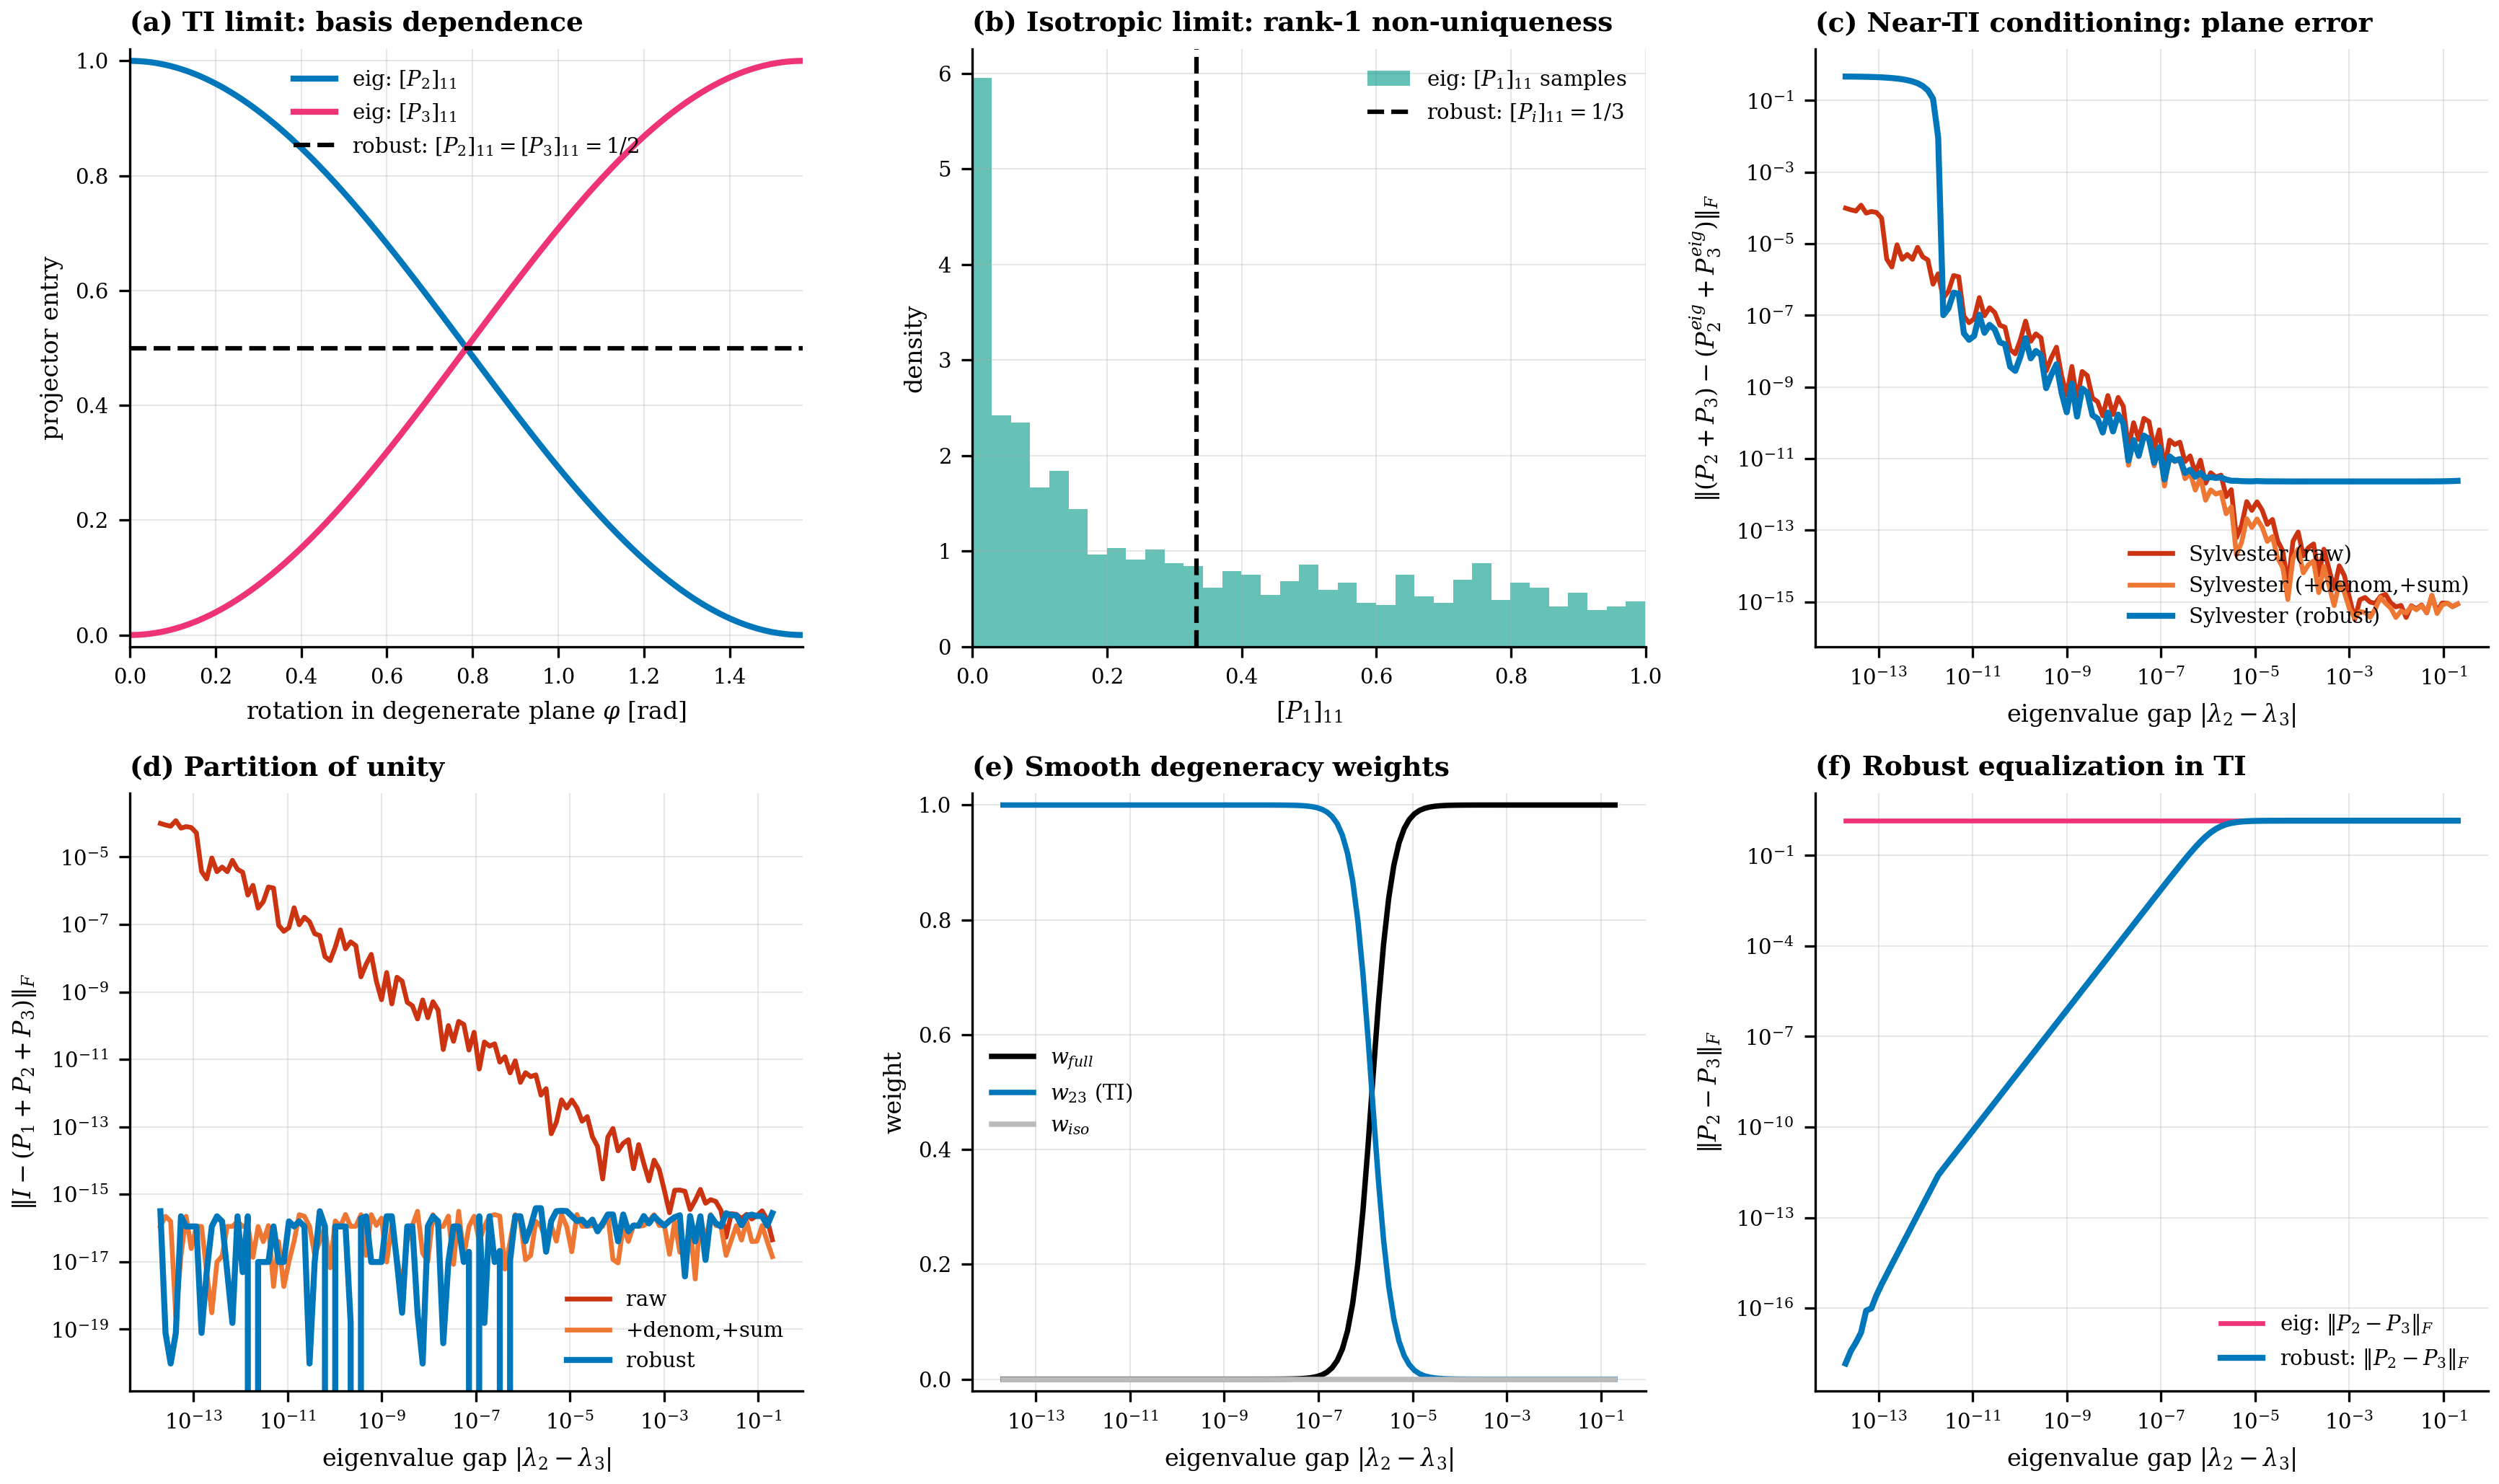
\includegraphics[width=\textwidth]{sylvester_projectors.png}
    \caption{Robust Sylvester projectors for symmetric $3\times3$ tensors.
(a) \textbf{TI limit (basis dependence):} In the transversely isotropic limit ($\lambda_2 \approx \lambda_3$), spectral projectors computed via eigendecomposition oscillate depending on the arbitrary choice of basis in the degenerate plane. The robust construction enforces a symmetric split, yielding a unique, invariant result.
(b) \textbf{Isotropic limit (non-uniqueness):} For equal eigenvalues, standard rank-one eigenprojectors are random (dependent on noise/basis). The robust limit correctly yields $\mathbf{I}/3$.
(c) \textbf{Conditioning near TI:} The raw Sylvester formula becomes singular as eigenvalue gaps vanish.
The robust method remains bounded; although the enforcement of the partition of unity distributes the regularization residual (leading to a finite approximation error in the transition regime), it ensures numerical stability and prevents divergence.
(d) \textbf{Partition of unity:} Explicitly enforcing $\sum \mathbf{P}_i=\mathbf{I}$ removes the drift associated with finite-precision arithmetic.
(e) \textbf{Regime blending:} Smooth weights transition from the full anisotropic formula to the TI split as the gap shrinks.
(f) \textbf{Robust equalization:} The robust construction forces $\|\mathbf{P}_2-\mathbf{P}_3\|_F\to0$ in the degenerate limit, effectively avoiding basis flips inherent to standard eigensolvers.}
    \label{fig:sylvester_projectors}
\end{figure}

Let $\mathbf{X}\in\mathbb{R}^{3\times 3}$ be a symmetric second-order tensor with (real) eigenvalues
$\{\lambda_1,\lambda_2,\lambda_3\}$, assumed available from an invariant-based closed-form procedure.
The spectral decomposition reads
\begin{equation}
\mathbf{X}=\sum_{i=1}^{3}\lambda_i\,\mathbf{P}_i,\qquad 
\mathbf{P}_i=\mathbf{n}_i\otimes \mathbf{n}_i,\qquad
\sum_{i=1}^{3}\mathbf{P}_i=\mathbf{I},
\end{equation}
where $\mathbf{P}_i$ are orthogonal projectors.
In anisotropic settings, the projectors can be obtained
without explicit eigenvectors by Sylvester's (Lagrange) interpolation.
\paragraph{Anisotropic (three distinct eigenvalues).}
For mutually distinct $\lambda_i$, the Sylvester projectors are
\begin{equation}
\label{eq:sylvester_Pi}
\mathbf{P}_i^{\mathrm{raw}}
=
\frac{\bigl(\mathbf{X}-\lambda_j\mathbf{I}\bigr)\bigl(\mathbf{X}-\lambda_k\mathbf{I}\bigr)}
{(\lambda_i-\lambda_j)(\lambda_i-\lambda_k)},
\qquad
(i,j,k)\ \text{a permutation of}\ (1,2,3).
\end{equation}
In finite precision arithmetic, near-degeneracy renders the denominators ill-conditioned. We therefore
regularize the denominators in a scale-aware manner.
Define the spherical/deviatoric split
$q=\tfrac13\mathrm{tr}(\mathbf{X})$ and $\mathbf{B}=\mathbf{X}-q\mathbf{I}$, and a tensor scale
\begin{equation}
\label{eq:scale_def}
s^2=\max\!\Bigl(q^2+\tfrac16\mathrm{tr}(\mathbf{B}^2),\,1\Bigr).
\end{equation}
For a scalar denominator $d$, we use the stabilized form
\begin{equation}
\label{eq:denom_stab}
d_{\mathrm{safe}}=\mathrm{sign}(d)\,\max\!\bigl(|d|,\varepsilon_d\,s^2\bigr),
\end{equation}
and replace $(\lambda_i-\lambda_j)(\lambda_i-\lambda_k)$ in~\eqref{eq:sylvester_Pi} by $d_{\mathrm{safe}}$.
To enforce the partition of unity exactly, we apply the symmetric correction
\begin{equation}
\label{eq:unity_fix}
\mathbf{P}_{\Sigma}=\sum_{i=1}^{3}\mathbf{P}_i^{\mathrm{raw}},\qquad
\mathbf{P}_{\mathrm{fix}}=\tfrac13(\mathbf{I}-\mathbf{P}_{\Sigma}),\qquad
\mathbf{P}_i^{\mathrm{full}}=\mathbf{P}_i^{\mathrm{raw}}+\mathbf{P}_{\mathrm{fix}}.
\end{equation}

\paragraph{Degeneracies: transverse and full isotropy.}
When two eigenvalues coalesce (transverse isotropy), only the projector onto the simple eigenvalue is unique,
whereas any orthonormal basis in the associated two-dimensional eigenspace is admissible.
To avoid arbitrary
basis selection, we introduce transverse-isotropic (TI) projector sets by splitting the degenerate subspace
symmetrically.
For example, if $\lambda_2\approx \lambda_3$ (pair $(23)$), we define
\begin{equation}
\label{eq:TI_split_23}
\mathbf{P}_1^{(23)}=\mathbf{P}_1^{\mathrm{full}},\qquad
\mathbf{P}_2^{(23)}=\mathbf{P}_3^{(23)}=\tfrac12\bigl(\mathbf{I}-\mathbf{P}_1^{\mathrm{full}}\bigr),
\end{equation}
and analogously for pairs $(12)$ and $(13)$ by selecting the corresponding unique index.
In the fully isotropic limit ($\lambda_1=\lambda_2=\lambda_3$), individual eigenprojectors are not defined;
we adopt the invariant convention
\begin{equation}
\label{eq:iso_split}
\mathbf{P}_1^{\mathrm{iso}}=\mathbf{P}_2^{\mathrm{iso}}=\mathbf{P}_3^{\mathrm{iso}}=\tfrac13\mathbf{I}.
\end{equation}

\paragraph{Smooth regime blending (robust transition).}
To obtain a numerically stable and differentiable transition between anisotropy, transverse isotropy, and
full isotropy, we use smooth ``gap'' indicators based on eigenvalue separations:
\begin{equation}
\label{eq:gap_indicator}
s_{ij}=\frac{\delta^2}{(\lambda_i-\lambda_j)^2+\delta^2},\qquad
\delta^2 = (\mathrm{tol}_{\mathrm{deg}}^2)\,s^2.
\end{equation}
Here, $s_{ij}\approx 0$ for well-separated eigenvalues and $s_{ij}\approx 1$ when $\lambda_i\approx\lambda_j$.
We define nonnegative weights for the anisotropic (full), three TI cases, and isotropy as
\begin{align}
w_{\mathrm{full}}&=(1-s_{12})(1-s_{23})(1-s_{13}), \nonumber\\
w_{12}&=s_{12}(1-s_{23})(1-s_{13}),\quad
w_{23}=s_{23}(1-s_{12})(1-s_{13}),\quad
w_{13}=s_{13}(1-s_{12})(1-s_{23}), \nonumber\\
w_{\mathrm{iso}}&=1-\bigl(w_{\mathrm{full}}+w_{12}+w_{23}+w_{13}\bigr),
\end{align}
so that $w_{\mathrm{full}}+w_{12}+w_{23}+w_{13}+w_{\mathrm{iso}}=1$ (a convex combination). The final robust projectors are then obtained as
\begin{equation}
\label{eq:final_blend}
\mathbf{P}_i
=
w_{\mathrm{full}}\,\mathbf{P}_i^{\mathrm{full}}
+w_{12}\,\mathbf{P}_i^{(12)}
+w_{23}\,\mathbf{P}_i^{(23)}
+w_{13}\,\mathbf{P}_i^{(13)}
+w_{\mathrm{iso}}\,\mathbf{P}_i^{\mathrm{iso}}.
\end{equation}
By construction, $\sum_i \mathbf{P}_i=\mathbf{I}$ and $\mathbf{P}_i=\mathbf{P}_i^{\mathsf T}$ hold in all regimes,
and the TI and isotropic limits avoid non-uniqueness of eigenvectors while preserving rotational invariance of the
degenerate subspaces.
\rev{To quantify the constitutive impact of this blending rule, we added a near-degenerate stress benchmark in which a fixed transversely isotropic log-fabric state is perturbed by symmetric noise of amplitude $\varepsilon_{\mathrm{noise}}$ and the resulting stress is compared with the exact TI limit. Using the constitutive law of \S\ref{subsec:mech-nd}, the naive rank-one eigendecomposition projectors, the raw Sylvester formula, and the denominator-regularized Sylvester formula all retain a finite relative stress error of approximately $1.3\times 10^{-1}$ at $\varepsilon_{\mathrm{noise}}=10^{-8}$, whereas the fully blended construction reduces the median error to $2.9\times 10^{-8}$ (\cref{fig:sylvester_stress_benchmark}). A separate sweep over the blending tolerance shows a broad low-error plateau for $\mathrm{tol}_{\mathrm{deg}}\in[10^{-6},10^{-5}]$; based on this benchmark, the default value used in the solver is set to $\mathrm{tol}_{\mathrm{deg}}=10^{-6}$. Smaller values fail to collapse reliably to the TI limit, while substantially larger values over-blend away from the genuinely anisotropic regime.}

\begin{figure}[htbp]
    \centering
    \safeincludegraphics[width=0.8\linewidth]{sylvester_stress_benchmark.png}
    \caption{\rev{Near-transverse-isotropy constitutive benchmark for projector robustness. (a) Relative stress error with respect to the exact TI limit versus perturbation amplitude $\varepsilon_{\mathrm{noise}}$ for eigendecomposition projectors, raw Sylvester projectors, denominator-regularized Sylvester projectors, and the fully robust blended construction. The robust method collapses to the TI limit as the perturbation vanishes, while the other variants retain a finite stress error. (b) Sensitivity of the robust method to the blending tolerance $\mathrm{tol}_{\mathrm{deg}}$ at $\varepsilon_{\mathrm{noise}}=10^{-8}$, showing a broad low-error plateau around $10^{-6}$--$10^{-5}$.}}
    \label{fig:sylvester_stress_benchmark}
\end{figure}
